% Label-free triplet supervision + InfoNCE schematic (figure 2).
% Build:  pdflatex training.tex   then   dvisvgm --pdf training.pdf
\documentclass[border=6pt]{standalone}
% Shared TikZ palette + primitive styles for the paper-style schematics.
% \input-ed by architecture.tex and training.tex. Colours ported from the old
% figures/toolkit.py PALETTE / EDGE / BAND_TINT.
\usepackage{tikz}
\usepackage{amsmath,amssymb,bm}
\usetikzlibrary{arrows.meta,positioning,fit,backgrounds,shadows.blur,calc}

% --- palette ---------------------------------------------------------------
\definecolor{ink}{HTML}{2B2B35}
\definecolor{muted}{HTML}{6B6B78}
\definecolor{line}{HTML}{9AA0AD}

\definecolor{clipFill}{HTML}{DBE7F5}\definecolor{clipEdge}{HTML}{7FA8D4}\definecolor{clipTint}{HTML}{EEF4FB}
\definecolor{queryFill}{HTML}{F5E6CC}\definecolor{queryEdge}{HTML}{D8B878}\definecolor{queryTint}{HTML}{FBF4E6}
\definecolor{trainFill}{HTML}{CDEACD}\definecolor{trainEdge}{HTML}{85C285}\definecolor{trainTint}{HTML}{EEF7EE}
\definecolor{negFill}{HTML}{F3D6D6}\definecolor{negEdge}{HTML}{DD9B9B}\definecolor{negTint}{HTML}{FCEEEE}
\definecolor{fuseFill}{HTML}{E8D6F3}\definecolor{fuseEdge}{HTML}{C298D8}\definecolor{fuseTint}{HTML}{F6EEFB}

\definecolor{posFill}{HTML}{D9EFD9}\definecolor{posEdge}{HTML}{5FAE5F}\definecolor{posInk}{HTML}{235C23}
\definecolor{negPillFill}{HTML}{F6D9D9}\definecolor{negPillEdge}{HTML}{D98989}\definecolor{negPillInk}{HTML}{7A2B2B}
\definecolor{goodGreen}{HTML}{2E7D32}
\definecolor{badRed}{HTML}{B3322F}
\definecolor{frostBlue}{HTML}{3D7CC0}
\definecolor{emberOrange}{HTML}{E8772E}
\definecolor{biton}{HTML}{7FA8D4}
\definecolor{bitflip}{HTML}{E0A52E}
\definecolor{avatarTile}{HTML}{F3F1EE}
\definecolor{avatarSil}{HTML}{B9BCC4}
\definecolor{badgeOk}{HTML}{2E9E4F}
\definecolor{badgeNo}{HTML}{CF4F4F}

% --- base styles -----------------------------------------------------------
\tikzset{
  every node/.style={font=\sffamily,text=ink},
  >={Stealth[round]},
  % rounded panel with soft shadow; role colours set via fill=...Fill, draw=...Edge
  panel/.style={rounded corners=4pt,draw,line width=0.9pt,blur shadow={shadow blur steps=5,
                shadow xshift=1.2pt,shadow yshift=-1.2pt,shadow opacity=28}},
  clip/.style ={panel,fill=clipFill, draw=clipEdge},
  query/.style={panel,fill=queryFill,draw=queryEdge},
  train/.style={panel,fill=trainFill,draw=trainEdge},
  neg/.style  ={panel,fill=negFill,  draw=negEdge},
  fuse/.style ={panel,fill=fuseFill, draw=fuseEdge},
  % a titled block: #1 = role style; use \blk macro below for title+subtitle text
  blk/.style 2 args={#1,align=center,inner sep=5pt},
  % stage band: dashed tinted backdrop drawn on the background layer
  band/.style={rounded corners=6pt,draw,line width=0.8pt,dash pattern=on 4pt off 3pt,
               inner sep=10pt},
  bandclip/.style ={band,fill=clipTint, draw=clipEdge},
  bandquery/.style={band,fill=queryTint,draw=queryEdge},
  bandtrain/.style={band,fill=trainTint,draw=trainEdge},
  bandneg/.style  ={band,fill=negTint,  draw=negEdge},
  bandfuse/.style ={band,fill=fuseTint, draw=fuseEdge},
  % signed pills
  pillpos/.style={rounded corners=7pt,fill=posFill,draw=posEdge,line width=0.9pt,
                  text=posInk,font=\sffamily\bfseries\small,inner sep=4pt},
  pillneg/.style={rounded corners=7pt,fill=negPillFill,draw=negPillEdge,line width=0.9pt,
                  text=negPillInk,font=\sffamily\bfseries\small,inner sep=4pt},
  % wires
  wire/.style={->,line width=1.1pt,ink},
  skipwire/.style={->,line width=1.0pt,muted,dash pattern=on 4pt off 3pt},
  % attribute-grid cells
  bitoff/.style={draw=line,line width=0.6pt,fill=white,minimum size=6pt,inner sep=0pt},
  biton/.style ={draw=line,line width=0.6pt,fill=biton,minimum size=6pt,inner sep=0pt},
  bitflip/.style={draw=bitflip,line width=1.5pt,minimum size=6pt,inner sep=0pt},
  wiretag/.style={font=\sffamily\scriptsize,text=muted,fill=white,inner sep=1.5pt,
                  fill opacity=0.85,text opacity=1},
  % --- layer-level (AlexNet/GoogLeNet-style) primitives ---
  lyr/.style={rounded corners=3pt,draw,line width=0.9pt,align=center,inner sep=4pt,
              font=\sffamily\small,fill=white,minimum height=0.78cm,minimum width=2.2cm},
  clipL/.style ={lyr,fill=clipFill, draw=clipEdge},
  queryL/.style={lyr,fill=queryFill,draw=queryEdge},
  trainL/.style={lyr,fill=trainFill,draw=trainEdge},
  negL/.style  ={lyr,fill=negFill,  draw=negEdge},
  fuseL/.style ={lyr,fill=fuseFill, draw=fuseEdge},
  % small elementwise-op node (\opn{$\oplus$})
  opn/.style={circle,draw=ink,line width=0.8pt,inner sep=0.5pt,font=\footnotesize,
              fill=white,minimum size=0.42cm},
  flow/.style={->,line width=1.0pt,ink},
}
% shape tag appended under a layer title: Title\dm{(B, 512)}
\newcommand{\dm}[1]{\\[1.5pt]{\ttfamily\scriptsize\color{muted}#1}}

% titled block: \blkbox{name}{role}{x,y}{width}{Title}{subtitle}
\newcommand{\blkbox}[6]{%
  \node[#2,minimum width=#4,align=center,inner sep=4pt] (#1) at (#3)
       {{\bfseries\small #5}\\[1pt]{\scriptsize\color{muted}#6}};}

% legend swatch
\newcommand{\swatch}[2]{\tikz[baseline=-0.5ex]\node[rounded corners=2pt,fill=#1,
  minimum width=9pt,minimum height=9pt,inner sep=0pt]{};~{\scriptsize #2}}

% placeholder face thumbnail: \avatar{name}{cx}{cy}{half-size}{edge colour}
\newcommand{\avatar}[5]{%
  \draw[rounded corners=2.5pt,fill=avatarTile,draw=#5,line width=1.1pt]
       (#2-#4,#3-#4) rectangle (#2+#4,#3+#4);
  \coordinate (#1) at (#2,#3);
  \begin{scope}
    \clip[rounded corners=2.5pt] (#2-#4,#3-#4) rectangle (#2+#4,#3+#4);
    \fill[avatarSil] (#2,#3+0.30*#4) circle ({0.55*#4});
    \fill[avatarSil] (#2,#3-0.55*#4) ellipse ({0.95*#4} and {0.72*#4});
  \end{scope}}
% pass/fail badge on the top-right of an avatar: \badge{cx}{cy}{half-size}{ok|no}
\newcommand{\badge}[4]{%
  \edef\bcol{\ifnum\pdfstrcmp{#4}{ok}=0 badgeOk\else badgeNo\fi}%
  \edef\bsym{\ifnum\pdfstrcmp{#4}{ok}=0 \noexpand\checkmark\else $\noexpand\times$\fi}%
  \draw[fill=\bcol,draw=white,line width=1.2pt] (#1+0.7*#3,#2+0.7*#3) circle ({0.42*#3});
  \node[text=white,font=\sffamily\bfseries\tiny] at (#1+0.7*#3,#2+0.7*#3) {\bsym};}

% 24-bit attribute grid (8 cols): \bitgrid{x}{y}{bit-string}{flip-list}
% bit-string: comma list of 0/1 (length 24); flip-list: comma indices (1-based) drawn highlighted
\newcommand{\bitgrid}[4]{%
  \begin{scope}[shift={(#1,#2)}]
    \foreach \bv [count=\i from 0] in {#3} {%
      \pgfmathtruncatemacro{\row}{div(\i,8)}\pgfmathtruncatemacro{\col}{mod(\i,8)}%
      \ifnum\bv=1\relax
        \node[biton]  (bc\i) at (0.24*\col,-0.24*\row) {};%
      \else
        \node[bitoff] (bc\i) at (0.24*\col,-0.24*\row) {};%
      \fi}%
    \edef\tmpflip{#4}%
    \ifx\tmpflip\empty\else
      \foreach \f in {#4} {\pgfmathtruncatemacro{\j}{\f-1}\node[bitflip] at (bc\j) {};}%
    \fi
  \end{scope}}

\begin{document}
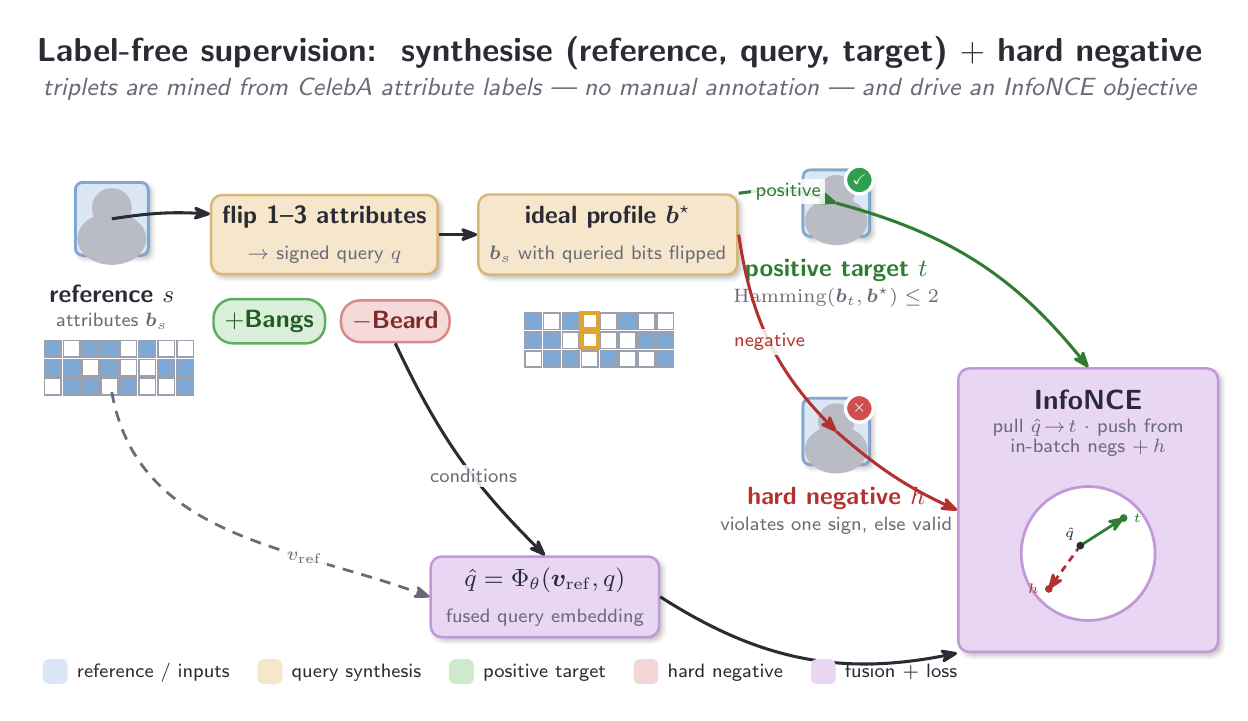
\begin{tikzpicture}[x=1cm,y=1cm]

  % ---- title ----
  \node[font=\sffamily\bfseries\large] at (7.75,8.3)
    {Label-free supervision:\ \ synthesise (reference, query, target) $+$ hard negative};
  \node[font=\sffamily\itshape\small,text=muted] at (7.75,7.85)
    {triplets are mined from CelebA attribute labels --- no manual annotation --- and drive an InfoNCE objective};

  % ================= reference =================
  \avatar{ref}{1.3}{6.2}{0.46}{clipEdge}
  \node[font=\sffamily\small\bfseries] at (1.3,5.25) {reference $s$};
  \node[font=\sffamily\scriptsize,text=muted] at (1.3,4.9) {attributes $\bm{b}_s$};
  \bitgrid{0.55}{4.55}{1,0,1,1,0,1,0,0,1,1,0,1,0,0,1,1,0,1,1,0,1,0,0,1}{}

  % ================= flip op =================
  \blkbox{flip}{query}{4.0,6.0}{2.6cm}{flip 1--3 attributes}{$\to$ signed query $q$}
  \node[pillpos] (qa) at (3.3,4.9) {$+$Bangs};
  \node[pillneg] (qb) at (4.9,4.9) {$-$Beard};

  % ================= ideal profile =================
  \blkbox{ideal}{query}{7.6,6.0}{2.8cm}{ideal profile $\bm{b}^\star$}{$\bm{b}_s$ with queried bits flipped}
  \bitgrid{6.65}{4.9}{1,0,1,0,0,1,0,0,1,1,0,0,0,0,1,1,0,1,1,0,1,0,0,1}{4,12}

  % ================= positive / hard negative =================
  \avatar{pos}{10.5}{6.4}{0.42}{trainEdge}\badge{10.5}{6.4}{0.42}{ok}
  \node[font=\sffamily\small\bfseries,text=goodGreen] at (10.5,5.55) {positive target $t$};
  \node[font=\sffamily\scriptsize,text=muted] at (10.5,5.2) {$\mathrm{Hamming}(\bm{b}_t,\bm{b}^\star)\le 2$};

  \avatar{hn}{10.5}{3.5}{0.42}{negEdge}\badge{10.5}{3.5}{0.42}{no}
  \node[font=\sffamily\small\bfseries,text=badRed] at (10.5,2.65) {hard negative $h$};
  \node[font=\sffamily\scriptsize,text=muted] at (10.5,2.3) {violates one sign, else valid};

  % ================= fusion + loss =================
  \blkbox{fuse}{fuse}{6.8,1.4}{2.9cm}{$\hat q=\Phi_\theta(\bm{v}_{\mathrm{ref}},q)$}{fused query embedding}

  \node[fuse,minimum width=3.3cm,minimum height=3.6cm] (loss) at (13.7,2.5) {};
  \node[font=\sffamily\bfseries] at (13.7,3.9) {InfoNCE};
  \node[font=\sffamily\scriptsize,text=muted] at (13.7,3.55) {pull $\hat q\!\to\! t$ $\cdot$ push from};
  \node[font=\sffamily\scriptsize,text=muted] at (13.7,3.3) {in-batch negs $+\,h$};
  % embedding inset
  \draw[fill=white,draw=fuseEdge,line width=1pt] (13.7,1.95) circle (0.85);
  \coordinate (qh) at (13.6,2.05);
  \coordinate (tp) at (14.15,2.4);
  \coordinate (hh) at (13.2,1.5);
  \draw[->,goodGreen,line width=1pt] (qh) -- (tp);
  \draw[->,badRed,line width=1pt,dash pattern=on 2.5pt off 2pt] (qh) -- (hh);
  \fill[ink] (qh) circle (1.4pt);\node[font=\bfseries\tiny,above left=-2pt] at (qh){$\hat q$};
  \fill[goodGreen] (tp) circle (1.4pt);\node[font=\bfseries\tiny,text=goodGreen,right=0pt] at (tp){$t$};
  \fill[badRed] (hh) circle (1.4pt);\node[font=\bfseries\tiny,text=badRed,left=0pt] at (hh){$h$};

  % ---- wires ----
  \draw[wire] (ref) to[bend left=6] (flip);
  \draw[wire] (flip) -- (ideal);
  \draw[wire,goodGreen,line width=1.1pt] (ideal.north east) to[bend left=14]
        node[wiretag,text=goodGreen,pos=0.5]{positive} (pos.west);
  \draw[wire,badRed,line width=1.1pt] (ideal.east) to[bend right=18]
        node[wiretag,text=badRed,pos=0.5]{negative} (hn.west);
  \draw[skipwire] (1.3,4.0) to[out=-80,in=160]
        node[wiretag,text=muted,pos=0.7]{$v_{\mathrm{ref}}$} (fuse.west);
  \draw[wire] (qb.south) to[bend right=10] node[wiretag,pos=0.6]{conditions} (fuse.north);
  \draw[wire] (fuse.east) to[bend right=22] (loss.south west);
  \draw[wire,goodGreen] (pos.south east) to[bend left=18] (loss.north);
  \draw[wire,badRed] (hn.east) to[bend right=8] (loss.west);

  % ================= legend =================
  \node[anchor=west,align=left,font=\sffamily] at (0.3,0.45)
    {\swatch{clipFill}{reference / inputs}\quad\swatch{queryFill}{query synthesis}\quad
     \swatch{trainFill}{positive target}\quad\swatch{negFill}{hard negative}\quad
     \swatch{fuseFill}{fusion $+$ loss}};

\end{tikzpicture}
\end{document}
